\chapter*{2022年\textsf{HDU}「大学物理1」期中试题解答}

\begin{minipage}{0.32\textwidth}
    \textbf{开课学院}：理学院
      
    \textbf{课程编码}：A0715011
\end{minipage}
\hfill
\begin{minipage}{0.32\textwidth}
    \textbf{解析制作}：\textsf{M.Xia@WeYoung}

    \textbf{\,\hologo{TeX}~排版}：\textsf{M.Xia}
\end{minipage}
\hfill
\begin{minipage}{0.15\textwidth}
    \centering
    \begin{tikzpicture}
        \node [inner sep=0] at (0,0) {
            \qrcode[height=3em,version=4]{https://qm.qq.com/q/mgD30uPiSs}};
        \fill [color=white,rounded corners=(sqrt(2)+2)/11*1em] (-.5em,-.5em) rectangle (.5em,.5em);
        \node [inner sep=0] at (0,0) {\color{MidnightBlue}\scriptsize\faIcon{qq}};
    \end{tikzpicture}

    \scriptsize\href{https://qm.qq.com/q/mgD30uPiSs}{\itshape 未央物理营}
\end{minipage}
\hfill
\begin{minipage}{0.15\textwidth}
    \centering
    \begin{tikzpicture}
        \node [inner sep=0] at (0,0) {
            \qrcode[height=3em,version=4]{http://weixin.qq.com/r/DBIABcHEqgnWKIVmb0eI}};
            \fill [color=white,rounded corners=(sqrt(2)+2)/11*1em] (-.5em,-.5em) rectangle (.5em,.5em);
        \node [inner sep=0] at (0,0) {\color{DarkGreen}\scriptsize\faIcon{weixin}};
    \end{tikzpicture}

    \scriptsize\href{http://weixin.qq.com/r/DBIABcHEqgnWKIVmb0eI}{\itshape 未央学社}
\end{minipage}

\section{选择题（每题3分，共30分）}

\begin{problem} % {平均速度与平均速率}
质点沿半径为$R$的圆周做匀速率运动，每$T$秒转一圈. 在$2T$时间间隔中其平均速度大小与平均速率大小分别为
\begin{tasks}(4)
    \task $2\pi R/T$，$2\pi R/T$
    \task $0$，$0$
    \task[\true] $0$，$2\pi R/T$
    \task $2\pi R/T$，$0$
\end{tasks}
\end{problem}
\begin{solution}
    位移$\Delta \bm x=0$，路程$s=2\times 2\pi R$. 所以$\abs{\overline{\bm v}}=\abs{\Delta\bm x/\Delta t}=0$，$\overline{v}=\Delta s/\Delta t=2\pi R/T$.
\end{solution}

\begin{problem} % {加速度}
在一个转动的齿轮上，一个齿尖$P$作半径为$R=1m$的圆周运动，其路程$s$随时间的变化规律为$s=2t+t^3$，则$t=\qty1\s$时齿尖$P$的加速度大小为
\begin{tasks}(4)
    \task $\qty6{\m/\s^2}$
    \task $\qty{16}{\m/\s^2}$
    \task[\true] $\qty{25.7}{\m/\s^2}$
    \task $\qty{25}{\m/\s^2}$
\end{tasks}
\end{problem}
\solute2
\begin{solution}
    $P$点的速度大小$v=\d s/\d t=\qty5{\m/\s}$；\textbf{切向}加速度大小$a_{\tau}=\d^2 s/\d t^2=\qty6{\m/\s^2}$；\textbf{法向}加速度大小$a_n=v^2/R=\qty{25}{\m/\s^2}$. 所以齿尖$P$的加速度大小$a=\sqrt{a_{\tau}^2+a_n^2}=\qty{25.7}{\m/\s^2}$.
\end{solution}

\begin{paracol}{2}
\begin{problem} % {动能定理，牛顿第二定律}
    如图所示，一质量为$m$的小球，由高$H$处沿光滑轨道由静止开始滑入环形轨道. 若$H$足够高，则小球在环最低点时环对它的作用力与小球在环最高点时环对他的作用力之差恰为小球重力的
    \begin{tasks}(4)
        \task $2$倍
        \task $4$倍
        \task[\true] $6$倍
        \task $8$倍
    \end{tasks}
    \switchcolumn\vspace*{\fill}\centering
    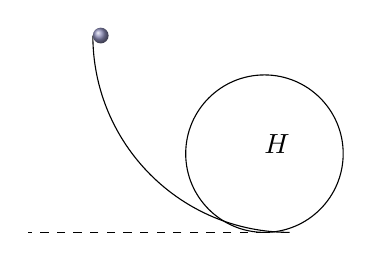
\begin{tikzpicture}
        \draw (0,0) circle (1);
        \draw [dashed] (0,-1) -- (-3,-1);
        \length{(-2.7,-1)}{(-2.7,1.5)}{$H$}{(0,.5)};
        \draw (-2.5,1.5) arc (-180:-90:2.5);
        \shade [ball color=MidnightBlue!50] (-2.4,1.5) circle (.1);
    \end{tikzpicture}\vspace*{\fill}
\end{problem}
\end{paracol}
\solute2
\begin{solution}
由动能定理$mgH=mv^2/2$得小球在运动到圆轨道底端、顶端时的速率分别为$v_1^2=2gH$，$v_2^2=2g(H-2R)$. 轨道的作用力和小球重力的合力提供向心力，在底端、顶端分别有$N_1-mg=mv_1^2/R$，$N_2+mg=mv_2^2/R$. 所以作用力之差为$N_1-N_2=2mg+m(v_1^2-v_2^2)/R=6mg$.
\end{solution}

\begin{problem}
一辆汽车从静止出发在平直公路上加速前进. 如果发动机的功率一定，下面哪种说法是正确的
\begin{tasks}(2)
    \task 汽车的加速度是不变的
    \task[\true] 汽车的加速度随时间减小
    \task 汽车的加速度与它的速度成正比
    \task 汽车的速度与它通过的路程成正比
\end{tasks}
\end{problem}
\begin{solution}
    由$a=\frac{F-f}{m}=\frac{P/v-f}{m}$可知汽车的加速度不断减小，由动能定理$Pt-fx=\frac{1}{2}mv^2-0$可知，$v$和$x$成非线性关系. 所以B选项正确.
\end{solution}

\begin{problem}
\begin{paracol}{2}
    如图所示，在光滑平面上有一个运动物体$P$，在$P$的正前方有一个连有弹簧的静止物体$Q$，弹簧的质量均不计，$P$与$Q$碰撞后$P$停止，$Q$以碰前$P$的速度运动. 在此碰撞过程中，弹簧压缩量最大时刻是
    \switchcolumn\centering
    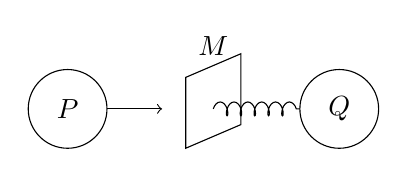
\begin{tikzpicture}
        \wall{(-.5,-.54)}{(3.95,-.7)};
        \draw (0,0) circle (.5) node {$P$};
        \draw [->] (.5,0) -- (1.2,0);
        \draw (1.5,.4) -- (1.5,-.5) -- (2.2,-.2) -- (2.2,.7) -- cycle node [above,midway] {$M$};
        \draw [decorate,decoration={coil,segment length=5pt}] (1.85,0) -- (2.95,0);
        \draw (3.45,0) circle (.5) node {$Q$};
    \end{tikzpicture}
\end{paracol}
\begin{tasks}(2)
    \task $P$的速度正好变为零时
    \task[\true] $P$与$Q$速度相等时
    \task $Q$正好开始运动时
    \task $Q$正好达到原来$P$的速度时
\end{tasks}
\end{problem}
\begin{solution}
    当$P$、$Q$发生``完全非弹性碰撞''时，二者共速，此时损失的动能最大，转换的弹簧弹性势能最大，弹簧压缩量也就最大.
\end{solution}

\begin{problem}
有一劲度系数为$k$的轻弹簧，原长为$l_0$，将它吊在天花板上. 当它下端挂一托盘平衡时，其长度变为$L_1$. 然后在托盘中放一重物，弹簧长度变为$l_2$. 则由$l_1$伸长为$l_2$的过程中，弹性力所作的功为
\begin{tasks}(4)
    \task $-\int_{l_1}^{l_2}kx\d x$
    \task $\int_{l_1}^{l_2}kx\d x$
    \task[\true] $-\int_{l_1-l_0}^{l_2-l_0}kx\d x$
    \task $\int_{l_1-l_0}^{l_2-l_0}kx\d x$
\end{tasks}
\end{problem}
\solute3
\begin{solution}
物体下落过程中所受恢复力为$F(x)=-kx$，$x$代表弹簧伸长量$l-l_0$. 所以弹性力做功$W=\int{F(x)\d x}=-\int_{l_1-l_0}^{l_2-l_0}kx\d x$.


\end{solution}
\begin{problem}
几个力同时作用在一个具有光滑固定转轴的刚体上，如果这几个力的矢量和为零，则此刚体
\begin{tasks}(2)
    \task 必然不会转动
    \task 转速必然不变
    \task 转速必然改变
    \task[\true] 转速可能不变，也可能改变
\end{tasks}
\end{problem}
\solute2
\begin{solution}
考虑两个大小相等，方向相反的力作用于刚体上：若两个力共线，则刚体所受到的外力矩为零，刚体的转速不变. 若两个力不共线，则刚体所受到的外力矩不为零，刚体的转速改变.
\end{solution}

\begin{problem}
人造地球卫星，绕地球作椭圆轨道运动，地球在椭圆的一个焦点上，则卫星的
\begin{tasks}(2)
    \task 动量不守恒，动能守恒
    \task 动量守恒，动能不守恒
    \task[\true] 对地心的角动量守恒，动能不守恒
    \task 对地心的角动量不守恒，动能守恒
\end{tasks}
\end{problem}
\solute1
\begin{solution}
卫星运动过程中受到的引力始终指向地球方向，所以受到的相对地球的合外力矩为零，但合外力不为零，所以角动量守恒；动量、动能均不守恒.
\end{solution}

\begin{problem}
带有$N$个电子的一个油滴质量为$m$，电子的电量的大小为$e$，在重力场中由静止开始下落，下落中穿越一均匀电场区域，欲使油滴在该区域中均匀下落，电场的方向和大小分别为
\begin{tasks}(4)
    \task 方向向上，$mg/Ne$
    \task[\true] 方向向下，$mg/Ne$
    \task 方向向上，$Ne/mg$
    \task 方向向下，$Ne/mg$
\end{tasks}
\end{problem}
\solute2
\begin{solution}
    油滴匀速下落，所受的合外力为零，即$mg=Ne\cdot E$，$E=mg/Ne$. 对于电子，电场方向应竖直向下以保证其所受的电场力方向竖直向上.
\end{solution}

\begin{problem} % {角动量}
\begin{paracol}{2}
    如图所示，一个小物体，位于光滑的水平桌面上，与一绳的一端相连结，绳的另一端穿过桌面中心的小孔$O$. 该物体原以角速度$\omega$在半径为$R$的圆周上绕$O$旋转，今令绳从小孔缓慢往下拉，则物体
    \switchcolumn\centering
    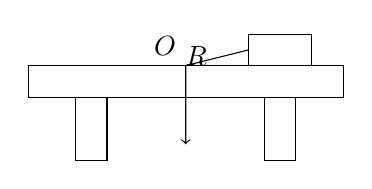
\begin{tikzpicture}[scale=.4]
        \draw (-5,0) rectangle (5,-1);
        \draw (-2.5,-1) rectangle (-3.5,-3);
        \draw (2.5,-1) rectangle (3.5,-3);
        \draw (2,0) rectangle (4,1);
        \draw [->] (2,.5) -- (0,0) node [above left] {$O$} -- (0,-2.5);
        \length{(0,1.5)}{(3,1.5)}{$R$}{(1,0)};
    \end{tikzpicture}
\end{paracol}
\begin{tasks}(2)
    \task 动能不变，动量改变
    \task 动量不变，动能改变
    \task 角动量不变，动量不变
    \task 角动量改变，动量改变
    \task![\true] 角动量不变，动能、动量都改变
\end{tasks}
\end{problem}
\solute2
\begin{solution}
    物块受力方向始终指向$O$点，所以对$O$点合外力矩为零，角动量守恒；但物体所受合外力不为零，所以动量、动能不守恒.
\end{solution}

\section{填空题}

\begin{problem}
一列火车以$\qty{36}{\km/\hour}$的速率向东行驶时相对于地面竖直下落的雨滴在列车的窗子上形成的雨迹偏离竖直方向$\qty{30}{\degree}$，则雨滴对地的速率是\ans{$10\sqrt{3}\unit{\m/\s}$}；相对列车的速率是\ans{$\qty{20}{\m/\s}$}.
\end{problem}
\solute2
\begin{solution}\leavevmode
    \begin{itemize}
        \item 火车速度$\bm v_1=10\bm i$，雨滴对地速度$\bm v_2=-b\bm j$，雨滴相对火车速度$\bm v_{21}=\bm v_2-\bm v_1=-10\bm i-b\bm j$.
        \item 车窗上雨迹偏离竖直方向$\qty{30}{\degree}$，雨相对火车速度与竖直方向夹角为$\qty{30}{\degree}$，即$10/b=\tan 30^\circ$.
        \item 所以雨滴对地速率$\abs{\bm v_2}=b=10\sqrt{3}\unit{\m/\s}$，相对于火车速率$\sqrt{b^2+10^2}=\qty{20}{\m/\s}$.
    \end{itemize}
\end{solution}

\begin{paracol}{2}
\begin{problem}
    质量为$m$的小球，用轻绳$AB$、$BC$连接，如图所示，其中$AB$水平，剪断绳$AB$前后的瞬间，绳$BC$中的张力比$T:T'=$\ans{$1:\cos^2\theta$}.
    \switchcolumn\vspace*{\fill}\centering
    \begin{tikzpicture}[scale=.6]
        \draw [ultra thick] (-2,2.5) -- (1.2,2.5);
        \draw [ultra thick] (-2,2.5) -- (-2,-.5);
        \draw (1,2.5) coordinate (c) node [above] {$C$} -- (0,0) coordinate (b) node [right] {$B$} node [above left] {$m$} -- (-2,0) node [left] {$A$};
        \draw [dashed] (1,2.5) -- (1,-.5) coordinate (d);
        \shade[ball color = MidnightBlue] (0,0) circle (.1);
        \draw [MidnightBlue,very thick,->] (0,0) -- (-.8,0);
        \draw [MidnightBlue,very thick,->] (0,0) -- (.8,2) node [left] {$T$};
        \draw [MidnightBlue,very thick,->] (0,0) -- (0,-2) node [right] {$mg$};
        \draw [MidnightBlue,very thick,->] (0,0) -- (.512,1.28) node [left] {$T'$};
        \pic["$\theta$",draw=DarkRed,ultra thick,angle eccentricity=1.5,angle radius=18]{angle=b--c--d};
    \end{tikzpicture}\vspace*{\fill}
\end{problem}\switchcolumn
\solute1
\begin{solution}    
    剪断前后，$m$分别沿竖直方向和绳方向受力平衡，即$T\cos\theta=mg$，$mg\cos\theta=T'$. 解得$T:T'=1:\cos^2\theta$.
\end{solution}
\end{paracol}

\begin{paracol}{2}
\begin{problem}
    如图所示一圆锥摆，质量为$m$的小球在水平面内以角速度$\omega$匀速转动. 在小球转动一周的过程中，小球动量增量的大小等于\ans{$0$}，小球所受绳子拉力的冲量大小等于\ans{$2\pi mg/\omega$}.
    \switchcolumn\vspace*{\fill}\centering
    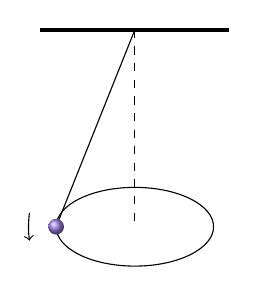
\begin{tikzpicture}
        \draw [ultra thick] (-1.2,2.5) -- (1.2,2.5);
        \draw [dashed] (0,2.5) -- (0,0);
        \draw (0,0) ellipse (1 and .5);
        \draw (0,2.5) -- (-1,0);
        \draw [->] ({-1.35*cos(7.5)},{1.35*sin(7.5)}) arc (172.5:187.5:1.35);
        \shade[ball color=blue!80!red!50] (-1,0) circle (.1);
    \end{tikzpicture}\vspace*{\fill}
\end{problem}
\switchcolumn
\solute1
\begin{solution}
    转动一周后小球的动量增量为$0$，所以小球所受重力的与绳子拉力的冲量大小相等，即$I_T=2\pi mg/\omega$.
\end{solution}
\end{paracol}

\begin{problem}
若作用于一力学系统上外力的合力为零，则外力的和力矩\ans{不一定}（``填一定''或``不一定''）为零；这种情况下力学系统的动量、角动量、机械能三个量中一定守恒的量是\ans{动量}.
\end{problem}

\begin{problem}
半径为$r=\qty{1.5}\m$的飞轮，初角速度$\omega_0=\qty{10}{\radian/\s}$，角加速度$\beta=\qty{-5}{\radian/\s^2}$. 则在$t=$\ans{$\qty4\s$}时角位移为零，而此时边缘上点的线速度$v=$\ans{$\qty{-15}{\m/\s}$}.
\end{problem}
\solute2
\begin{solution}
    飞轮的角位移的表达式为$\theta=\omega_0 t+\beta t^2/2$，令$\theta=0$得$t=\qty4\s$时角位移为零. 此时边缘上点的线速度大小为$v=r(\omega_0+\beta t)=\qty{-15}{\m/\s}$.
\end{solution}

\begin{paracol}{2}
\begin{problem}
    如图所示，一匀质木球固结在一细棒下端，且可绕水平光滑固定轴$O$
    转动. 今有一子弹沿着与水平面成一角度的方向击中木球而嵌于其中，则在此击中过程中，木球、子弹、细棒的\ans{水平方向动量 \& 对$O$的点角动量}守恒，木球被击中后棒和球升高的过程中，木球、子弹、细棒、地球系统的\ans{机械能}守恒.
    \switchcolumn\centering
    \begin{tikzpicture}[scale=.75]
        \draw (0,0) node [left] {$O$} -- (0,-2);
        \draw (0,-2.6) circle (.6);
        \draw [dashed] (0,0) -- ({sqrt(2)},{-sqrt(2)});
        \draw [rotate around={45:(0,0)},dotted] (0,-2.6) circle (.6);
        \draw [dashed,->] (-1.2,-1.4) -- (0,-2.6);
        \draw [dashed] (-1.2,-2.6) -- (0,-2.6);
    \end{tikzpicture}
\end{problem}
\end{paracol}
\begin{solution}
    击中过程中木球、子弹、细棒三者中的外力只有木球受到沿着杆方向的力，而此力对三者的力矩为$0$，所以三者水平方向动量、对$O$点的角动量守恒；升高过程中木球、子弹、细棒、地球之间只有保守力做功，所以机械能守恒.
\end{solution}

\begin{problem}
    由一根绝缘细线围成的边长为$l$的正方形线框，使它均匀带电，其电荷线密度为$\lambda$，则在正方形中心处的电场强度的大小$E=$\ans{$0$}.
\end{problem}
\solute3
\begin{solution}
    由对称性可知，四边在中心产生的合场强为$0$.
\end{solution}
\solute*{为节约资源，本试题计算题部分不提供演算区域，请自备稿纸，或在下页边缘书写.}

\section{计算题（共46分）}

\begin{paracol}{2}
\begin{problem}
    质量为$m$的物体系于长度为$R$的绳子的一个端点上，在竖直平面内绕绳子另一端点（固定）作圆周运动. 设$t$时刻物体瞬时速度的大小为$v$，绳子与竖直向上的方向成$\theta$角，如图所示. 求
    \begin{enumerate}
        \item $t$时刻绳中的张力$T$和物体的切向加速度$a_\tau$.
        \item 说明在物体运动过程中$a_\tau$的大小和方向如何变化？
    \end{enumerate}
    \switchcolumn\vspace*{\fill}\centering
    \begin{tikzpicture}[scale=.9]
        \draw [dotted] (0,0) circle ({sqrt(2)}) coordinate (o) node [right] {$O$};
        \draw [->] (0,0) -- (-1,1) coordinate (b) node [midway,below left] {$R$} node [left] {$m$} -- (-1.5,.5) node [left] {$v$};
        \shade [ball color=MidnightBlue!50] (-1,1) circle (.1);
        \draw [dashed] (0,0) -- (0,{sqrt(2)}) coordinate (a);
        \pic["$\theta$",draw=DarkRed,ultra thick,angle eccentricity=1.8,angle radius=12]{angle=a--o--b};
    \end{tikzpicture}\vspace*{\fill}
\end{problem}
\end{paracol}
\begin{solution}\leavevmode
\begin{enumerate}
    \item 选取自然坐标系，分别列小球切向和法向的牛顿运动定律
    \[mg\sin\theta=ma_{\tau},\ T+mg\cos\theta=\frac{mv^2}{R}\]
    解得$T=mv^2/R-mg\cos\theta$，$a_{\tau}=g\sin\theta$.
    \item 
    \begin{multicols}{2}
        \begin{itemize}
            \item $0\leq\theta\leq\pi/2$，$a_{\tau}$增大，方向与$\bm v$相同.
            \item $\pi/2\leq\theta\leq\pi$，$a_{\tau}$减小，方向与$\bm v$相同.
            \item $\pi\leq\theta\leq3\pi/2$，$a_{\tau}$增大，方向与$\bm v$相反.
            \item $\frac{3}{2}\pi\leq\theta\leq 2\pi$，$a_{\tau}$减小，方向与$\bm v$相反.
        \end{itemize}
    \end{multicols}
\end{enumerate}
\end{solution}

\begin{problem}
一质点沿$x$轴运动，其加速度$a$与位置坐标$x$的关系为$a=2+6x^3$ (SI)，如果质点在原点处的速度为$v_0$，试求其在任意位置$x$处的速度.
\end{problem}
\begin{solution}
    由链式法则得$a=\d v/\d t=\d v/\d x\cdot\d x/\d t=v\d v/\d x$. 分离变量$v\d v=a\d x$，积分得
    \[\int v\d v=\int(2+6x^3)\d x,\ \frac{1}{2}v^2=2x+\frac{3}{2}x^4+C\]
带入初态$v=v_0$，$x=0$得$C=v_0^2/2$. 所以任意位置的速度表达式为$v=\sqrt{v_0^2+4x+3x^4}$ (SI).
\end{solution}

\begin{problem}
    一质点沿直线运动，其坐标$x$与时间$t$有关系$x=A\e^{-\beta t}\cos\omega t$ (SI).
    \begin{tasks}[label=\arabic*.](2)
        \task 求任意时刻$t$质点的速度.
        \task 求质点通过原点的时刻$t$.
    \end{tasks}
\end{problem}
\begin{solution}\leavevmode
    \begin{tasks}[label=\arabic*.](2)
        \task $v=\odv xt=-A\beta\e^{-\beta t}\cos\omega t-\omega A\e^{-\beta t}\sin\omega t$.
        \task 令$x=0$，得$t=\pi/2\omega+k\pi/\omega$，$k\in\mathbb N$.
    \end{tasks}
\end{solution}

\begin{paracol}{2}
\begin{problem}
    一质量为$m$的物体悬于一条轻绳的一端，绳另一端绕在一轮轴的轴上，如图所示. 轴水平且垂直于轮面，其半径为$R$，整个装置架在光滑的固定轴承之上. 当物体从静止释放后，在时间$t$内下降了一段距离$S$. 试求整个轮轴的转动惯量（用$m$、$R$、$t$和$S$表示）.
    \switchcolumn\vspace*{\fill}\centering
    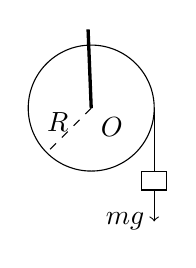
\begin{tikzpicture}[scale=.8]
        \wall{(-1.25,1.25)}{(1.25,1.45)};
        \draw (0,0) circle (1) node [below right] {$O$};
        \draw [very thick] (0,0) -- (-.05,1.25);
        \draw (1,0) -- (1,-1);
        \draw (.8,-1) rectangle (1.2,-1.3);
        \draw [->] (1,-1.3) -- (1,-1.8) node [left] {$mg$};
        \draw [dashed] (0,0) -- ({-sqrt(2)/2},{-sqrt(2)/2}) node [above,near end] {$R$};
    \end{tikzpicture}\vspace*{\fill}
\end{problem}    
\end{paracol}
\begin{solution}\leavevmode
    \begin{itemize}
        \item 设绳子张力$T$，对物块列牛顿运动定律$mg-T=ma=mR\beta$.
        \item 转盘所受合力矩$M=TR$，由转动定律$TR=I\beta$.
        \item 由以上可知$a$为常数，物块作匀变速直线运动，所以有$S=at^2/2$.
        \item 联立以上四式，解得整个轮轴的转动惯量为$I=mgR^2t^2/2S-mR^2$.
    \end{itemize}
\end{solution}

\begin{paracol}{2}
\begin{problem}
    如图所示，一长为$\qty{10}{\cm}$的均匀带正电细杆，其上电荷量为$\qty{1.5e-8}{\C}$，试求在杆的延长线上距杆的端点$\qty5{\cm}$处的$P$点的电场强度.
    \switchcolumn\vspace*{\fill}\centering
    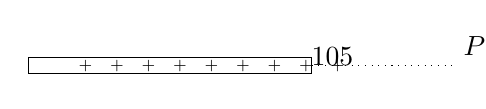
\begin{tikzpicture}
        \draw (-3.6,-.1) rectangle (0,.1);
        \draw [dotted] (0,0) -- (1.8,0);
        \length{(-3.6,-.5)}{(0,-.5)}{$\qty{10}\cm$}{(1,0)};
        \length{(0,-.5)}{(1.8,-.5)}{$\qty5\cm$}{(1,0)};
        \foreach \x in {0,...,8}
            \node [xshift=.4*\x cm] at (-3.4,0) {$\scriptscriptstyle+$};
        \shade[ball color=blue!80!red!50] (1.8,0) circle (.06);
        \node [anchor=south east] at (1.8,0) {$P$};
    \end{tikzpicture}\vspace*{\fill}
\end{problem}
\end{paracol}
\begin{solution}
设杆长$l$，$P$点距离杆右端距离为$d$，杆上的电荷线密度$\lambda=q/L$. 以杆左端为原点，以向右为正方向建立坐标轴.

对杆上$x\sim x+\d x$的一段线元，其电荷量$\d q=\lambda\d x$，与$P$点的距离为$l+d-x$，在$P$处产生的场强大小为$\d E=\d q/4\pi\epsilon_0(l+d-x)^2$，对其积分得
\[E=\int_0^l\d E=\int_0^l\frac{1}{4\pi\epsilon_0}\frac{\lambda\d x}{(l+d-x)^2}=\qty{1.8e4}{\N/\C}\]
方向沿$x$轴正向.
\end{solution}

\begin{paracol}{2}
\begin{problem}
    如图所示，一水平刚性轻杆，质量不计，杆长$l=\qty{20}\cm$，其上穿有两个小球，初始时，两小球相对杆中心$O$对称放置，与$O$的距离$d=\qty5\cm$，二者之间用细线拉紧. 现在让细杆绕通过中心$O$的竖直固定轴作匀角速的转动，转速为$\qty2{\radian/\s}$，再烧断细线让两球向杆的两端滑动. 不考虑转轴的和空气的摩擦，当两球都滑至杆端时，试求杆的角速度.
    \switchcolumn\vspace*{\fill}\centering
    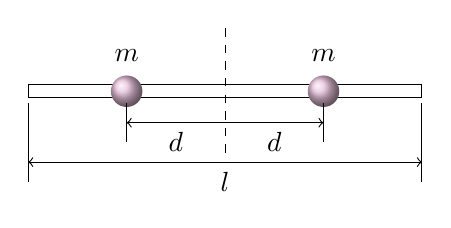
\begin{tikzpicture}
        \draw (-2.5,.08) rectangle (2.5,-.08);
        \draw [dashed] (0,.8) -- (0,-.8);
        \shade[ball color=blue!40!red!25] (-1.25,0) circle (.2);
        \shade[ball color=blue!40!red!25] (1.25,0) circle (.2);
        \draw (-2.5,-.15) -- (-2.5,-1.15);
        \draw (2.5,-.15) -- (2.5,-1.15);
        \draw (-1.25,-.15) -- (-1.25,-.65);
        \draw (1.25,-.15) -- (1.25,-.65);
        \draw [<->] (-1.25,-.4) -- (1.25,-.4);
        \draw [<->] (-2.5,-.9) -- (2.5,-.9);
        \node [anchor=north] at (0,-.9) {$l$};
        \node [anchor=north] at (-.625,-.4) {$d$};
        \node [anchor=north] at (.625,-.4) {$d$};
        \node [anchor=south] at (-1.25,.25) {$m$};
        \node [anchor=south] at (1.25,.25) {$m$};
    \end{tikzpicture}\vspace*{\fill}
\end{problem}    
\end{paracol}
\begin{solution}
由角动量守恒$2md^2\omega_1=2m(l/2)^2\omega_2$，解得杆的角速度为$\omega_2=\qty{0.5}{\radian/\s}$.
\end{solution}

\begin{paracol}{2}
\begin{problem}
    一物体与斜面间的摩擦系数$\mu=0.20$，斜面固定，倾角$\alpha=45^{\circ}$. 现给予物体一初速率$v_0=\qty{10}{\m/\s}$，使它沿斜面向上滑，如图所示. 求
    \begin{enumerate}
        \item 物体能够上升的最大高度$h$.
        \item 物体达到最高点后，沿斜面返回到原出发点时的速率$v$.
    \end{enumerate}
    \switchcolumn\vspace*{\fill}\centering
    \begin{tikzpicture}[scale=.6]
        \draw (0,0) coordinate (o) -- (5,0) coordinate (a) -- (5,5) coordinate (b) -- cycle;
        \draw [rotate around={45:(0,0)}] (0,0) rectangle + ({sqrt(2)},{.5*sqrt(2)});
        \draw [rotate around={45:(3,3)}] (3,3) rectangle + ({sqrt(2)},{.5*sqrt(2)});
        \draw [->] (.75,1.25) -- (1.75,2.25) node [above] {$v_0$};
        \length{(3.25,3)}{(3.25,0)}{$h$}{(0,-.75)};
        \pic["$\alpha$",draw=DarkRed,ultra thick,angle eccentricity=1.8,angle radius=12]{angle=a--o--b};
    \end{tikzpicture}\vspace*{\fill}
\end{problem}
\end{paracol}
\begin{solution}\leavevmode
\begin{enumerate}
    \item 上升过程中物块受摩擦力大小为$\mu mg\cos\alpha$，对物块列动能定理
    \[mgh+\mu mg\cos\alpha\frac{h}{\sin\alpha}=\frac12mv^2\]
    解得$h=v_0^2/2g(1+\mu \cot\alpha)=\qty{25}\m/6$.
    \item 全过程中，重力是保守力，所以做的总功为$0$. 考虑摩擦力做功，由动能定理
    \[2\mu mg\cos\alpha\frac{h}{\sin\alpha}=\frac12mv_0^2-\frac12mv^2\]
    解得$\displaystyle v=\sqrt{v_0^2-4\mu g\cos\alpha h/\sin\alpha}=\frac{10\sqrt6}3\unit{\m/\s}$.
\end{enumerate}
\end{solution}